\documentclass[a4paper,12pt]{article} % тип документа

% Поля страниц
\usepackage[left=2.5cm,right=2.5cm,
    top=2cm,bottom=2cm,bindingoffset=0cm]{geometry}
    
%Пакет дял таблиц   
\usepackage{multirow} 
    
%Отступ после заголовка    
\usepackage{indentfirst}


% Рисунки
\usepackage{floatrow,graphicx,calc}
\usepackage{wrapfig}

%%% Работа с картинками
\usepackage{graphicx}  % Для вставки рисунков
\graphicspath{{images/}}  % папки с картинками
\setlength\fboxsep{3pt} % Отступ рамки \fbox{} от рисунка
\setlength\fboxrule{1pt} % Толщина линий рамки \fbox{}
\usepackage{wrapfig} % Обтекание рисунков и таблиц текстом

% Создаём новый разделитель
\DeclareFloatSeparators{mysep}{\hspace{1cm}}

% Ссылки?
\usepackage{hyperref}
\usepackage[rgb]{xcolor}
\hypersetup{				% Гиперссылки
    colorlinks=true,       	% false: ссылки в рамках
	urlcolor=blue          % на URL
}


%  Русский язык
\usepackage[T2A]{fontenc}			% кодировка
\usepackage[utf8]{inputenc}			% кодировка исходного текста
\usepackage[english,russian]{babel}	% локализация и переносы

% Математика
\usepackage{amsmath,amsfonts,amssymb,amsthm,mathtools}

%%% Дополнительная работа с математикой
\usepackage{amsmath,amsfonts,amssymb,amsthm,mathtools} % AMS
\usepackage{icomma} % "Умная" запятая: $0,2$ --- число, $0, 2$ --- перечисление

% Что-то 
\usepackage{wasysym}


\begin{document}
\begin{center}
	\footnotesize{ФЕДЕРАЛЬНОЕ ГОСУДАРСТВЕННОЕ АВТОНОМНОЕ ОБРАЗОВАТЕЛЬНОЕ 			УЧРЕЖДЕНИЕ ВЫСШЕГО ОБРАЗОВАНИЯ}\\
	\footnotesize{МОСКОВСКИЙ ФИЗИКО-ТЕХНИЧЕСКИЙ ИНСТИТУТ\\(НАЦИОНАЛЬНЫЙ 			ИССЛЕДОВАТЕЛЬСКИЙ УНИВЕРСИТЕТ)}\\
	\footnotesize{ФИЗТЕХ-ШКОЛА ФИЗИКИ И ИССЛЕДОВАНИЙ им. ЛАНДАУ\\}
	\hfill \break
	\hfill \break
	\hfill \break
	\hfill \break
\end{center}

\begin{center}   
    \hfill \break
	\hfill \break
	\hfill \break
	\hfill \break    \hfill \break
	\hfill \break
	\hfill \break
	\hfill \break
    \hfill \break
    \hfill \break
	\hfill \break
	\large{Лабораторная работа № 2.1.4\\\textbf{Определение теплоёмкости твёрдых тел}}\\
	\begin{flushright}
		Плотникова Анастасия Александровна\\
		Группа Б02-406
	\end{flushright}
	\hfill \break
	\hfill \break
	\hfill \break
\end{center}
\hfill \break
\hfill \break
\hfill \break
\hfill \break
\hfill \break
\hfill \break
\hfill \break
\hfill \break
\hfill \break
\hfill \break
\hfill \break
\hfill \break
\hfill \break
\begin{center}
	Долгопрудный, 2025 г.
\end{center}
\thispagestyle{empty}
\newpage
	\textbf{Цель работы:}\\ 
  1) прямое измерение кривых нагревания ($T_{heat}(t)$) и охлаждения ($T_{cool}(t)$) пустого калориметра и системы «калориметр + твердое тело»; \\
  2) определение коэффициента теплоотдачи стенок калориметра; \\
  3) определение теплоемкости пустого калориметра и удельной теплоемкости твердого тела.
	\hfill \break
	
	\textbf{В работе используются:}\\ 
  калориметр с нагревателем и термометром сопротивления; \\
  универсальный вольтметр В7-78/3 в режиме омметра, \\
  измеритель температуры: \\
  — термопара K-типа, \\
  — универсальный вольтметр В7-78/2, \\
  источник питания GPS-72303, \\
  универсальные вольтметры В7-78/3 (в режиме амперметра), \\
  KEITHLEY (в режиме вольтметра) для измерения мощности нагревателя, \\
  компьютерная программа АКИП для сопряжения персонального компьютера и универсальных вольтметров В7-78/2 и В7-78/3.
	
\section*{Теоретическая справка}

При подведении к телу количества тепла $\Delta Q$ за время $\Delta t$, изменение температуры $\Delta T$ связано с теплоёмкостью $C$ выражением:

\[
C = \frac{\Delta Q}{\Delta T}
\]

С учётом теплопотерь:

\[
C \Delta T = P \Delta t - \lambda (T - T_k) \Delta t
\]

В дифференциальной форме уравнения нагревания и охлаждения:

\[
C \frac{dT_{\text{heat}}(t)}{dt} = P - \lambda (T_{\text{heat}}(t) - T_k(t))
\]

\[
C \frac{dT_{\text{cool}}(t)}{dt} = -\lambda (T_{\text{cool}}(t) - T_k(t))
\]

Связь между сопротивлением термометра и температурой:

\[
R_T = R_{273} \left[ 1 + \alpha (T - 273) \right]
\]

Для пересчёта сопротивлений, измеренных при комнатной температуре $T_k$, используется выражение:

\[
R_{273} = \frac{R_k}{1 + \alpha (T_k - 273)}
\]

Тогда, подставив, получим:

\[
T(R_T) = \frac{R_T}{R_k} \cdot \frac{1 + \alpha (T_k - 273)}{1 + \alpha (T - 273)} \cdot 273
\]

В эксперименте используется температурный коэффициент сопротивления меди $\alpha = 4.28 \cdot 10^{-3}$ град$^{-1}$.

При охлаждении калориметра ($P = 0$) уравнение принимает вид:

\[
C \frac{dT}{dt} = -\lambda (T - T_k)
\]

Интегрируя от начального момента $t = 0$ до $t$, получим:

\[
T(t) = (T_0 - T_k) e^{-\frac{\lambda}{C}t} + T_k
\]

Из графика зависимости $\ln(T - T_k)$ от $t$ можно найти наклон, равный $-\lambda/C$.

При нагревании калориметра ($P \neq 0$):

\[
C \frac{dT}{dt} = P - \lambda (T - T_k)
\]

Интегрирование даёт:

\[
T(t) = \left(1 - e^{-\frac{\lambda}{C}t} \right) \cdot \frac{P}{\lambda} + T_k
\]

В «удобной точке», когда $T = T_k$, получаем простую формулу для определения теплоемкости:

\[
C = \frac{P}{\left. \frac{dT}{dt} \right|_{T = T_k}}
\]

Также можно использовать значения производных при одной и той же температуре $T$ на кривых нагревания и охлаждения. Тогда:

\[
C = \frac{P \left( \frac{dT}{dt} \right)_{\text{cool}}}{\left( \frac{dT}{dt} \right)_{\text{heat}} - \left( \frac{dT}{dt} \right)_{\text{cool}}}
\]

\[
\lambda = \frac{P}{\left( \frac{dT}{dt} \right)_{\text{heat}} - \left( \frac{dT}{dt} \right)_{\text{cool}}} \cdot \left( \frac{dT}{dt} \right)_{\text{cool}}
\]

Если $T_k$ одинаково для обеих кривых, формулы упрощаются:

\[
C = \frac{P}{\left( \frac{dT}{dt} \right)_{\text{heat}} - \left( \frac{dT}{dt} \right)_{\text{cool}}}
\]

\[
\lambda = \frac{P}{\left( \frac{dT}{dt} \right)_{\text{heat}} - \left( \frac{dT}{dt} \right)_{\text{cool}}} \cdot \left( \frac{dT}{dt} \right)_{\text{cool}}
\]


\section*{Экспериментальная установка}

Схема установки изображена на рисунке (\ref{fig:setup}). 

Установка включает калориметр с пенопластовой изоляцией, размещенный в ящике из многослойной фанеры. 

Внутренние стенки калориметра выполнены из материала с высокой теплопроводностью, с усеченными конусами для обеспечения плотного контакта. 

Выталкивание образца происходит через винт в донышке. В стенку калориметра вмонтированы спираль нагревателя и терморезистор.
\begin{figure}[h!]
  \centering
  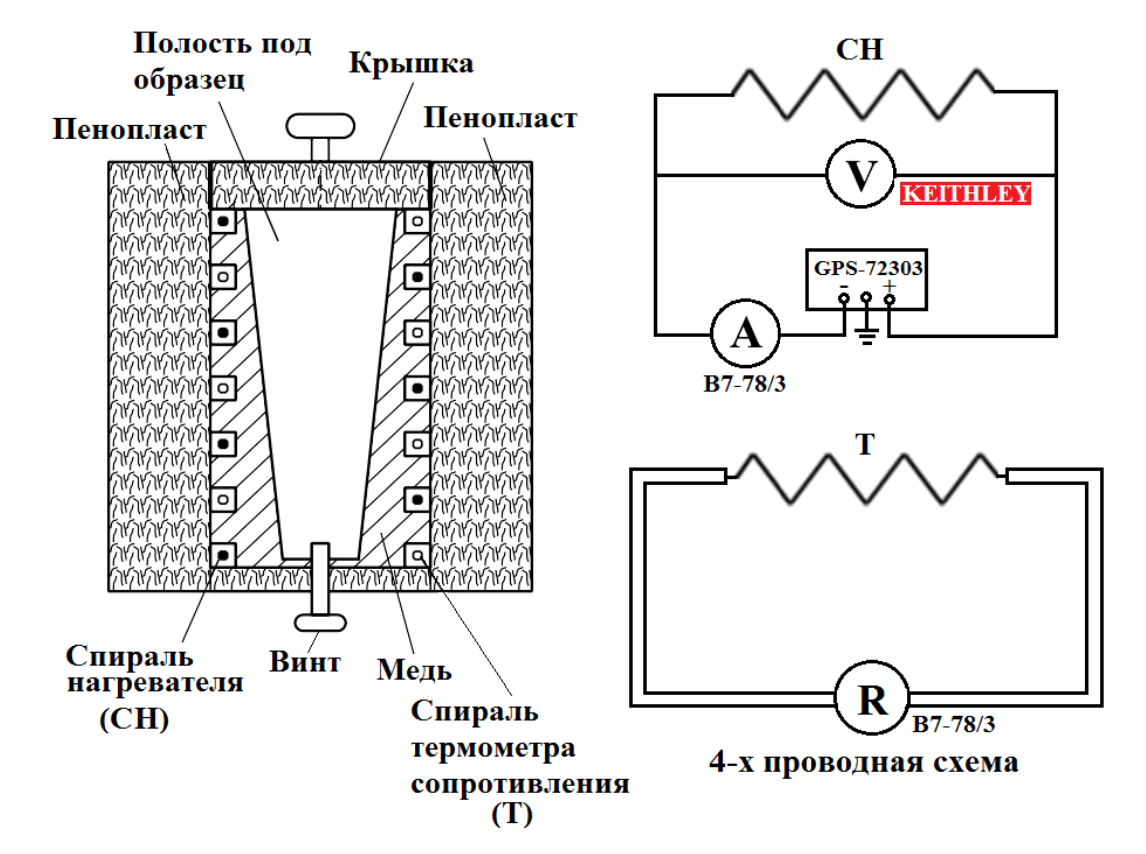
\includegraphics[scale=0.6]{setup.png}
  \caption{Схема установки}
  \label{fig:setup}
\end{figure}

\section*{Ход работы}

\begin{center}
  \textsf{I. Подготовка к эксперименту}
\end{center}

\begin{enumerate}
    \item Включим в сеть измерительные приборы: источник питания GPS-72303 (кнопка «POWER», кнопку «OUTPUT» не будем включать!), два универсальных вольтметра В7-78/3 (кнопка «Сеть»), универсальный вольтметр В7-78/2 (кнопка «Сеть»), универсальный вольтметр KEITHLEY (кнопка «POWER»). Установим требуемые режимы работы мультиметров. Универсальный вольтметр В7-78/2 переведём в режим измерения температуры с помощью термопары K-типа (последовательное нажатие кнопок «преф» и «темп»). Универсальный вольтметр В7-78/3 (1) переведём в режим измерения сопротивления по четырёхточечной схеме (последовательное нажатие кнопок «преф» и «$\Omega2$»), ещё один универсальный вольтметр В7-78/3 (2) переведём в режим измерения постоянного тока (последовательное нажатие кнопок «преф» и «U=»). Убедимся, что универсальный вольтметр KEITHLEY при включении автоматически перейдёт в режим измерения постоянного напряжения (V DC).

    \item Включим компьютер (ноутбук MSI). Убедимся в том, что он не подключён к интернету и запустим с рабочего стола программу АКИП B7-78 PT-Tool.

    \item Убедимся, что программа видит универсальные вольтметры В7-78/2 и В7-78/3, предназначенные соответственно для измерения временной зависимости комнатной температуры (термопара К-типа) в градусах $^\circ$C и сопротивления спирали термометра (Т) в Омах.

    \item Из меню «Настройки» выберем пункт «Настройки устройства». Для каждого прибора из списка устройств выберем необходимый режим, путём нажатия соответствующих кнопок подтвердим и загрузим настройки вольтметров. Нажмём «Выход».

    \item Из меню «Настройки» выберем пункт «Настройки Режима». Отметим режим сбора «Несколько устройств». В разделе «параметры» для каждого из вольтметров выберем необходимый «цвет графика» и номер файла записи (например, Record1 и Record2). Поставим галочку «Сохранить» и нажмём ОК.

    \item В главном окне программы выберем «разряд» (цену деления измеряемой величины по оси ординат) и «смещение» графика в целых единицах измеряемой величины относительно горизонтальных курсоров 1 и 2 (каждому курсору соответствует свой прибор). Курсоры 1 и 2 вместе с соответствующими графиками переместим кнопками «Up» и «Dn». Затем выберем «скорость» записи (временной шаг) и «точки» (количество точек по оси времени). 

    \item Подготовим лабораторный журнал для фиксации ключевых действий и времени (по часам ноутбука). Будем записывать только важные события, чтобы потом соотнести их с графиками.

    \item Нажмём кнопку «Старт» в верхнем левом углу программы и не будем выключать её до завершения работы. Через 40 секунд на графике появятся кривые температуры (красная) и сопротивления (синяя). Ось времени направлена справа налево. Будем использовать графики для контроля хода эксперимента. Цифровые значения извлечём позже из CSV-файлов.
\end{enumerate}


\begin{center}
  \textsf{II. Проведение измерений}
\end{center}

\begin{enumerate}
    \item Охладим калориметр до температуры на 2–5 $^\circ$C ниже комнатной. Температуру калориметра проконтролируем по калибровочной кривой $T(R)$ терморезистора (график рядом с установкой). Для этого вставим в калориметр охлаждённый латунный конус. Через 3–4 минуты, после того как температура в калориметре начнёт медленно расти, извлечём конус и вернём его в ёмкость с охлаждённой водой. Подождём ещё 3–4 минуты.

    \item При неизменной мощности нагревателя определим зависимость сопротивления терморезистора $R_{\text{heat}}(t)$ от времени для пустого калориметра. Для этого замкнём цепь спирали нагревателя СН (нажмём кнопку «OUTPUT» на источнике GPS-72303, должна загореться зелёная лампочка). Будем следить за ростом температуры калориметра. Как только она превысит комнатную на 8–9 $^\circ$C (через 25–30 минут), отключим нагреватель (повторно нажмём кнопку «OUTPUT», зелёная лампочка погаснет).

    \item Определим зависимость $R_{\text{cool}}(t)$ при охлаждении пустого калориметра. Будем продолжать наблюдение до снижения температуры на 1–2 $^\circ$C по сравнению с моментом отключения нагревателя. 

    \item Снова охладим калориметр до температуры на 2–5 $^\circ$C ниже комнатной, используя латунный образец (как в п. 1). Вставим исследуемое тело в калориметр и повторим измерения $R_{\text{heat}}(t)$ и $R_{\text{cool}}(t)$, как в пп. 2–3.

    \item Проведём измерения для двух образцов — из железа и алюминия.

    \item По завершении всех измерений нажмём кнопку «Стоп» в программе АКИП. В меню «Регистратор» выберем пункт «Просмотр Записи». Сохраним файлы Record1 и Record2 в папку «Лаба 214» на рабочем столе и на флешку. Присвоим файлам узнаваемые имена.
\end{enumerate}

\begin{center}
  \textsf{III. Обработка результатов измерений}
\end{center}

\begin{enumerate}
    \item Откроем CSV-файлы Record1 и Record2 в программе Excel. Каждый файл содержит две колонки: первая — время в формате \texttt{чч:мм:сс}, вторая — показания: в °C (термопара) или в Ом (терморезистор).

    \item Разделим данные по столбцам: выделим первую колонку, затем выберем «Данные» → «Текст по столбцам» → «С разделителями» → выберем «Запятая» → «Готово».

    \item Преобразуем формат времени в секунды: удалим заголовки, очистим первую колонку, зададим первый элемент как 0, второй — как 1. Выделим оба, протянем вниз до конца таблицы, чтобы получить последовательность времени $t = 0, 1, 2, \dots$

    \item Пересчитаем значения сопротивления терморезистора $R_T$ в температуру $T(R_T)$ по калибровочной формуле:

    \[
    T(R_T) = 14.584 \cdot R_T + 39.355 \quad \text{(установка 1)}
    \]
    \[
    T(R_T) = 14.378 \cdot R_T + 39.355 \quad \text{(установка 2)}
    \]

    \item Пересчитаем температуру окружающей среды $T_k$ из градусов Цельсия в Кельвины по формуле:

    \[
    T_k[\text{K}] = T_k[^\circ\text{C}] + 273.15
    \]

    \item Построим графики $T_{\text{heat}}(t)$, $T_{\text{cool}}(t)$ и $T_k(t)$. Сопоставим участки с лабораторными записями и определим кривые для пустого калориметра и с образцами.

    \item Построим график зависимости:
    \[
    \ln(T_{\text{cool}}(t) - T_k) \text{ от } t
    \]
    Исключим начальный нелинейный участок. На линейном участке определим тангенс наклона — это $\lambda / C$.

    \item Используя выражение:
    \[
    T(t) = (T_0 - T_k) e^{-\lambda t / C} + T_k
    \]
    и найденное ранее отношение $\lambda / C$, определим коэффициент теплоотдачи $\lambda$, затем теплоёмкость $C$ пустого калориметра.

    \item Повторим пункты 6–8 для образцов из железа и алюминия. Найдём полную теплоёмкость системы и определим теплоёмкость тел как:

    \[
    C_{\text{Fe}} = C_{\text{Fe+cal}} - C_{\text{cal}}, \quad C_{\text{Al}} = C_{\text{Al+cal}} - C_{\text{cal}}
    \]

    \item Альтернативно определим $C$ и $\lambda$ дифференциальными методами:
    \begin{itemize}
        \item В точке $T = T_k$:
        \[
        C = \frac{P}{\left. \frac{dT}{dt} \right|_{T = T_k}}
        \]
        \item В одинаковых точках $T$ на кривых нагрева и охлаждения:
        \[
        C = \frac{P \left( \frac{dT}{dt} \right)_{\text{cool}}}{\left( \frac{dT}{dt} \right)_{\text{heat}} - \left( \frac{dT}{dt} \right)_{\text{cool}}}
        \]
        \[
        \lambda = \frac{P}{\left( \frac{dT}{dt} \right)_{\text{heat}} - \left( \frac{dT}{dt} \right)_{\text{cool}}} \cdot \left( \frac{dT}{dt} \right)_{\text{cool}}
        \]
    \end{itemize}

    \item Сравним результаты, полученные интегральным и дифференциальным методами, с табличными значениями. Проанализируем точность и возможные источники погрешностей.
\end{enumerate}

\section*{Вывод}
\end{document}
